%
% File: chap02.tex
% Author: Tengxiang Li
%
\chapter{Chapter Title}
\label{chap:02}
\setlength{\parskip}{1em}
%

\begin{equation}
    Q = \frac{1}{h^{3N}N!}\int\int{e^{-{\beta}H(p,q)}}dpdq
\end{equation}
%
\begin{equation}
    H(p,q) = \sum_{i=1}^{N}\frac{p_i^2}{2m_i}+V(q)
    \label{hamiltonian}
\end{equation}
%
%

\begin{figure}[H]
{
\centering  
\begin{subfigure}{0.3 \textwidth}
    \centering
    {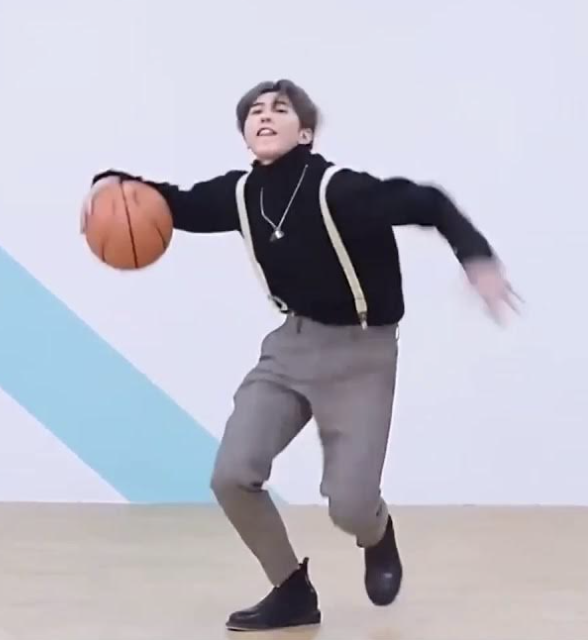
\includegraphics[width=\textwidth]{figures/fig02/2.5.png}
    \caption{}\label{Fig.2.1.a}}
\end{subfigure}
%
\begin{subfigure}{0.3 \textwidth}
    \centering
    {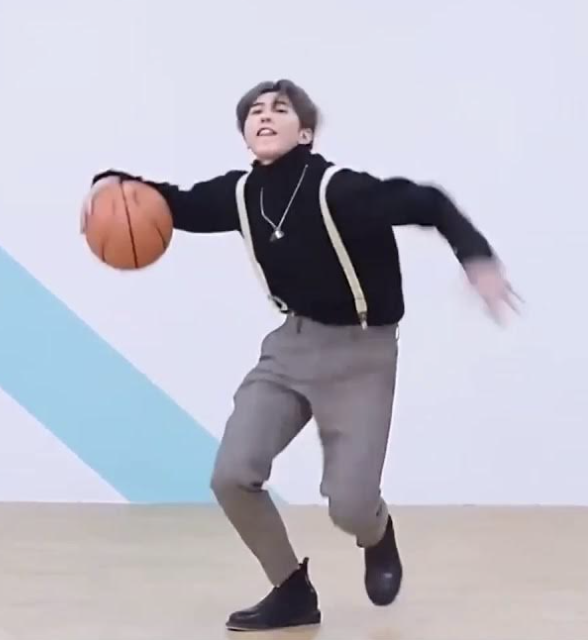
\includegraphics[width=\textwidth]{figures/fig02/2.5.png}
    \caption{}\label{Fig.2.1.b}}
\end{subfigure}
%
\begin{subfigure}{0.3 \textwidth}
    \centering
    {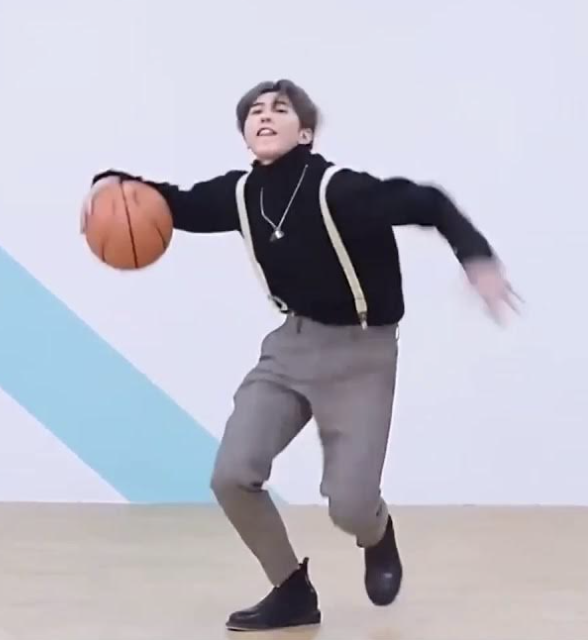
\includegraphics[width=\textwidth]{figures/fig02/2.5.png}
    \caption{}\label{Fig.2.1.c}}
\end{subfigure}

\caption{Description of this figure}
\label{Fig.2.1}
}
\end{figure}
%
\section{Section title}
AITU AITU
% \subsection{Subsection title}
% AITU AITU

%
% File: sec 2-1.tex
% Author: Tengxiang Li
%
\section{Section title}
AITU AITU
\subsection{Subsection title}
AITU AITU
%
